% chktex-file 44

\section{\large Ejercicio 2. Solución de sistemas de ecuaciones lineales $3\times3$.}

\[
    \begin{aligned}
        2x+6y+2z=10\\
        3x-2y-4z=-3 \\
        5x-y-z=4
    \end{aligned}
\]

Resuelva el sistema de ecuaciones lineales seleccionado \textbf{(literal A, B, C, D o E)} utilizando el método de eliminación de Gauss-Jordán. Asegúrese de validar el resultado utilizando herramientas computacionales como GeoGebra, Symbolab u otras. Incluya la comprobación del resultado y explique detalladamente el procedimiento de eliminación paso a paso.

\textbf{Solución en GeoGebra}
\begin{figure}[ht!]
    \centering
    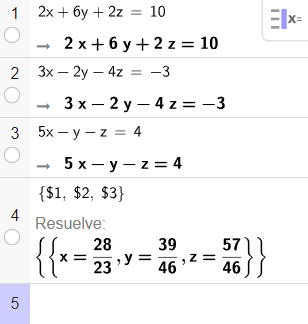
\includegraphics{geogebra2.png}
\end{figure}

\textbf{Solución algebraica}
\[
    \left(
        \begin{array}{ccc|c}
            \textbf{x} & \textbf{y} & \textbf{z} & \textbf{i} \\
            2 & 6 & 2 & 10 \\
            3 & -2 & -4 & -3 \\
            5 & -1 & -1 & 4 \\
        \end{array}
    \right)
    \begin{pmatrix}
        1 & 0 & 0 \\
        0 & 1 & 0 \\
        0 & 0 & 1 \\
    \end{pmatrix}
\]

\[
    \begin{aligned}
        \left(
            \begin{array}{ccc|c}
                2 & 6 & 2 & 10 \\
                3 & -2 & -4 & -3 \\
                5 & -1 & -1 & 4 \\
            \end{array}
        \right)
        & \frac{f1}{2} \\ \\
        \left(
            \begin{array}{ccc|c}
                1 & 3 & 1 & 5 \\
                3 & -2 & -4 & -3 \\
                5 & -1 & -1 & 4 \\
            \end{array}
        \right)
        & -3f1+f2 \\ \\
        \begin{array}{ccc|c}
            -3 & -9 & -3 & -15 \\
            3 & -2 & -4 & -3 \\
            \hline
            0 & -11 & -7 & -18 \\
        \end{array}
        & = 
        \left(
            \begin{array}{ccc|c}
                1 & 3 & 1 & 5 \\
                0 & -11 & -7 & -18 \\
                5 & -1 & -1 & 4 \\
            \end{array}
        \right)
        -5f1+f3 \\ \\
        \begin{array}{ccc|c}
            -5 & -15 & -5 & -25 \\
            5 & -1 & -1 & 4 \\
            \hline
            0 & -16 & -6 & -21 \\
        \end{array}
        & = 
        \left(
            \begin{array}{ccc|c}
                1 & 3 & 1 & 5 \\
                0 & -11 & -7 & -18 \\
                0 & -16 & -6 & -21 \\
            \end{array}
        \right)
        \frac{f2}{-11} \\ \\
    \end{aligned}
\]

\[
  \begin{aligned}
    \left(
        \begin{array}{ccc|c}
            1 & 3 & 1 & 5 \\
            0 & 1 & \frac{7}{11} & \frac{18}{11} \\
            0 & -16 & -6 & -21 \\
        \end{array}
    \right)
    & 16f2+f3 \\ \\
    \begin{array}{ccc|c}
        0 & 16 & \frac{112}{11} & \frac{288}{11} \\
        0 & -16 & -6 & -21 \\
        \hline
        0 & 0 & \frac{46}{11} & \frac{57}{11}
    \end{array}
    & =
    \left(
        \begin{array}{ccc|c}
            1 & 3 & 1 & 5 \\
            0 & 1 & \frac{7}{11} & \frac{18}{11} \\
            0 & 0 & \frac{46}{11} & \frac{57}{11} \\
        \end{array}
    \right)
    \frac{f3}{\frac{46}{11}} \\ \\
    \left(
        \begin{array}{ccc|c}
            1 & 3 & 1 & 5 \\
            0 & 1 & \frac{7}{11} & \frac{18}{11} \\
            0 & 0 & 1 & \frac{57}{46} \\
        \end{array}
    \right)
    & f2-\frac{7}{11}f3 \\ \\
    \begin{array}{ccc|c}
        0 & 1 & \frac{7}{11} & \frac{18}{11} \\
        0 & 0 & \frac{-7}{11} & \frac{399}{506} \\
        \hline
        0 & 1 & 0 & \frac{39}{46}
    \end{array}
    & =
    \left(
        \begin{array}{ccc|c}
            1 & 3 & 1 & 5 \\
            0 & 1 & 0 & \frac{39}{46} \\
            0 & 0 & 1 & \frac{57}{46} \\
        \end{array}
    \right)
    & f1-f3 \\ \\
  \end{aligned}  
\]

\[
  \begin{aligned}
    \begin{array}{ccc|c}
        1 & 3 & 1 & 5 \\
        0 & 0 & -1 & \frac{-57}{46} \\
        \hline
        1 & 3 & 0 & \frac{173}{46}
    \end{array}
    & =
    \left(
        \begin{array}{ccc|c}
            1 & 3 & 0 & \frac{173}{46} \\
            0 & 1 & 0 & \frac{39}{46} \\
            0 & 0 & 1 & \frac{57}{46} \\
        \end{array}
    \right)
    & f1-3f2 \\ \\
    \begin{array}{ccc|c}
        1 & 3 & 0 & \frac{173}{46} \\
        0 & -3 & 0 & \frac{-117}{46} \\
        \hline
        1 & 0 & 0 & \frac{28}{23}
    \end{array}
    & =
    \left(
        \begin{array}{ccc|c}
            1 & 0 & 0 & \frac{28}{23} \\
            0 & 1 & 0 & \frac{39}{46} \\
            0 & 0 & 1 & \frac{57}{46} \\
        \end{array}
    \right)
    & f1-3f2 \\ \\
  \end{aligned}  
\]

\begin{center}
    \textbf{Solución:} \(\left(\frac{28}{23}, \frac{39}{46}, \frac{57}{46}\right)\)
\end{center}